\documentclass[main.tex]{subfiles}
\begin{document}
\section{Widley Linear Filtering and Adaptive Spectrum Estimation}

\subsection{Complex LMS and Widely Linear Modelling}

In what has previously been analysed, only real time signals have been considered. However, complex-valued signals are a crucial way of representing informations in communications, signal proccessing, biomedial signal processing and related fields. Complex values are either created by design (such as in communications), or are a convenient way of describing two dimensional environemnt parameters (such as wind direction). 

Applying similar methods for coefficient estimation in the complex space is possible with a few modifications to the original algorithms. The Complex-Least Mean Squared (CLMS) algorithm is one of the more widely used algorithms, and is defined in much the same way as the LMS algorithm introduced in Section 3. 

However, the CLMS algorithm is not guaranteed to capture correct filter coefficients for all situations. When considering a non-circular, the resulting estimation for the filter coefficients from the CLMS does not capture second order dependencies. 

\subsubsection{Comparison of CLMS and ACLMS}

As the CLMS algorithm does neccecssarily capture second order statistical relationships, the Augmented CLMS (ACLMS) is introduced. This is able to capture the second order relationships by including a second set of coefficients which acts on the \textbf{conjugate} of the input vector $\textbf{x}$. The algorithm is defined as;

\begin{align*}
\hat{y}(n) &= \textbf{h}^H(n)\textbf{x}(n) + \textbf{g}^H(n)\textbf{x}^*(n) \numberthis \label{eq-4-1-a-yest}\\
e(n) &= y(n) - \hat{y}(n)\\
\textbf{h}(n+1) &= \textbf{h}(n) + \mu e^*(n) \textbf{x}(n)\\
\textbf{g}(n+1) &= \textbf{g}(n) + \mu e^*(n) \textbf{x}^*(n)
\end{align*}

The effectiveness of the CLMS and ALMS is tested by considering the following WLMA(1) input. A model order of 1 is passed to both the CLMS and ACLMS algorithms, with the results for model error (learning curve) show in figure~\ref{fig:q4_1_a}

\begin{equation}
y(n) = x(n) + b_1x(n-1) + b_2x(n=1)\ \ \ \ \ \ x \sim \mathcal{N}(0,1)
\end{equation}

where $x$ is complex, circular WGN, $b_1 = 1.5+1j$, $b_2  = 2.5-0.5j$.

\begin{figure}[H]
	\centering 
	\resizebox{0.9\textwidth}{!}{\input{matlabimages/4-1-a.tikz}}
	\caption{ACLMS and CLMS learning curves for WLMA(1)}
	\label{fig:q4_1_a}
\end{figure}

As the CLMS cannot properly capture the underlying data, the error at steady state remains at around $10dB$. However, the ACLMS is able to perfectly match the system, and the error at steady state tends towards 0; which in $dB$ tends towards $-\infty$.

\subsubsection{Bivariate Wind Data}

As well as estimating filter coefficients for direct WLMA processes, the CLMS and ACLMS algorithms can be used to predict real life data. Three sets of wind data (One for each low, medium and high wind strenght) are passed through each algorithm to attempt to model and predict future wind patterns.


\begin{figure}[H]
	\centering
	\includegraphics[width=0.8\textwidth]{images/4-1-b-1.pdf}
	\caption{Scatter Plots for Bivariate wind data of low (left), medium (center) and high (right) wind regimes}
	\label{fig:q4_1_b}
\end{figure}


From the scatter plots of the wind data (Figure \ref{fig:q4_1_b}), it can be extrapolated that the CLMS is sufficient for low wind data, as it appears to be more circular. However, medium and high wind strength appears less circular, indicating that the CLMS might not be able to fully follow the model. 

To investiage the performance of the CLMS and the ACLMS algorithms for the wind data, the steady state error averaged over 100 iterations is captured for a number of orders and learning coefficient values. From the results in fig~\ref{fig:q4_1_b_2}, it can be said that the ACLMS of order 3 is best for the low wind data, 

\begin{figure}[H]
	\centering 
	\resizebox{0.9\textwidth}{!}{\input{matlabimages/4-1-b-2.tikz}}
	\caption{Model Prediction for the Bivariate wind data. Error is the Mean Square Steady State Error calculated over the last 100 iterations}
	\label{fig:q4_1_b_2}
\end{figure}



\subsubsection{Three Phased Power Systems}

To investiaget the effect of biased versus unbiased three phased power systems, a matlab function {\tt p4\_three\_phase\_power} is introduced. The inputs here allow the definition of $V_a, V_b, V_c$, as well as $\phi, \Delta_b, \Delta_c$. The output of the function is the Clarke voltage, calculated through the Clarke Transform.  

The Clarke voltage is defined as

\begin{align*}
v(n) &= A(n)e^{j(2 \pi \frac{f_0}{f_s}n + \phi)} + B(n)e^{-j(2 \pi \frac{f_0}{f_s}n + \phi)}, \numberthis \label{eq-4-1-c-unbal}\\
where\ \ A(n) &= \frac{\sqrt{6}}{6}\left(V_a(n) + V_b(n)e^{j\Delta_b} + V_c(n)e^{j\Delta_c}\right)\\
and\ \ B(n) &= \frac{\sqrt{6}}{6}\left(V_a(n) + V_b(n)e^{-j(\Delta_b+2\pi/3)} + V_c(n)e^{-j(\Delta_c-2\pi/3)}\right)
\end{align*}

which simplifies to the following in the situation where the system is balanced, as $B(n)$ becomes 0.

\begin{equation}
v(n) = \sqrt{\frac{3}{2}} V e^{j(2 \pi \frac{f_0}{f_s}n + \phi)} \label{eq-4-1-c-bal}
\end{equation}


\begin{figure}[H]
	\centering 
	\resizebox{0.4\textwidth}{!}{\input{matlabimages/4-1-c.tikz}}
	\caption{Circularity plot for a balanced and an unbalanced power system}
	\label{fig:q4_1_c}
\end{figure}

When plotting the circularity diagrams of both a balanced and unbalanced system, it can be seen that only a balanced system will have perfectly round circle, whereas an unbalanced one will not. This property can be used to identify a fault in a given power system, as a non-perfect circle implies an unbalanced power system, which implies a fault.



\subsubsection{Clarke Voltage Frequency from Filter Coefficients}


The frequency of the Clarke Voltage can be extracted from the filter coefficients of the CLMS or the ACLMS. Two seperate situations are investigated: the strictly linear (Equation~\ref{eq-4-1-d-first}) and the widely linear (Equation~\ref{eq-4-1-d-second}) models.

\begin{align}
v(n+1) &= h^*(n)v(n) \label{eq-4-1-d-first}\\
v(n+1) &= h^*(n)v(n) + g^*(n)v^*(n) \label{eq-4-1-d-second}
\end{align}

\paragraph{For the strictly linear model,} equation~\ref{eq-4-1-c-bal} is used to find expressions for $v(n+1)$ and $v(n)$. These are substituted into equation~\ref{eq-4-1-d-first} to give

\begin{align*}
\sqrt{\frac{3}{2}} V e^{j(2 \pi \frac{f_0}{f_s}(n+1) + \phi)} &= h^*(n)\sqrt{\frac{3}{2}} V e^{j(2 \pi \frac{f_0}{f_s}n + \phi)}\\
e^{j(2 \pi \frac{f_0}{f_s}n + \phi)}e^{j(2 \pi \frac{f_0}{f_s})} &= h^*(n) e^{j(2 \pi \frac{f_0}{f_s}n + \phi)}\\
e^{j(2 \pi \frac{f_0}{f_s})} &= h^*(n) \\
arg(e^{j(2 \pi \frac{f_0}{f_s})}) &= arg(h^*(n)) \\
2 \pi \frac{f_0}{f_s} &= arctan\left(\frac{\Im(h^*(x))}{\Re(h^*(x))}\right) \\
f_0 &= - \frac{f_s}{2\pi} arctan\left(\frac{\Im(h(x))}{\Re(h(x))}\right) \\
\end{align*}

\paragraph{For the widely linear model,} the equations \ref{eq-4-1-c-unbal} and \ref{eq-4-1-d-second} are used to gather terms for $v(n+1)$ and $\hat{v}(n+1)$. The coefficients for both of these terms are equated to extrapolate the value of $f_0$ \cite{Xia2012} 

\begin{align*}
v(n+1) &= A(n+1)e^{j2\pi\frac{f_0}{f_s}}e^{j(2\pi  \frac{f_0}{f_s}n+\phi)} + B(n+1)e^{-j2\pi\frac{f_0}{f_s}}e^{-j(2\pi  \frac{f_0}{f_s}n+\phi)}\\
\hat{v}(n+1) &= h^*(n)\left(A(n)e^{j(2\pi\frac{f_0}{f_s}n+\phi)} + B(n)e^{-j(2\pi\frac{f_0}{f_s}n+\phi)}\right) + g^*(n)\left(A^*(n)e^{-j(2\pi\frac{f_0}{f_s}n+\phi)} + B^*(n)e^{j(2\pi\frac{f_0}{f_s}n+\phi)}\right)\\
&= \left[h^*(n)A(n) + g^*(n)B^*(n)\right] e^{j(2\pi\frac{f_0}{f_s}n+\phi)} + \left[h^*(n)B(n) + g^*(n)A^*(n)\right] e^{-j(2\pi\frac{f_0}{f_s}n+\phi)}
\end{align*}

At steady state, we can make two assumptions; Firstly, $A(n) \simeq A(n+1)$ and $B(n) \simeq B(n+1)$. Secondly, $v(n+1) \simeq \hat{v}(n+1)$. With these two assumptions, we can equate the first and second right hand side (RHS) terms,to find the two equations for the term $e^{j2\pi\frac{f_0}{f_s}}$;

\begin{align*}
e^{j2\pi\frac{f_0}{f_s}} &= \frac{A(n)h^*(n) + B^*(n)g^*(n)}{A(n+1)} \simeq \frac{A(n)h^*(n) + B^*(n)g^*(n)}{A(n)} \\
e^{-j2\pi\frac{f_0}{f_s}} &= \frac{A^*(n)g^*(n) + B(n)h^*(n)}{B(n+1)} \simeq \frac{A^*(n)g^*(n) + B(n)h^*(n)}{B(n)}\\
\left[e^{-j2\pi\frac{f_0}{f_s}}\right]^* &= e^{j2\pi\frac{f_0}{f_s}} =  \frac{A(n)g(n) + B^*(n)h(n)}{B^*(n)}
\end{align*}

Thus, we get

\begin{align*}
e^{j2\pi\frac{f_0}{f_s}} &= h^*(n) + \frac{B^*(n)}{A(n)}g^*(n)\\
e^{j2\pi\frac{f_0}{f_s}} &= h(n) + \frac{A(n)}{B^*(n)}g(n)
\end{align*}

It can be shown that $A(n)$ will always be real, and that $B(n)$ is complex. Therefore, $B^*(n)/A(n) = \left(B(n)/A(n)\right)^*$. If we consider $a(n) = (B(n)/A(n))^*$, and equate the two equations above,

\begin{align*}
h^*(n) + a(n)g^*(n) = h(n) + \frac{1}{a(n)}g(n)\\
a^2(n)\left[g^*(n)\right] + a(n)\left[h^*(n) - h(n)\right] + \left[-g(n)\right] &= 0\\
a^2(n)\left[g^*(n)\right] + a(n)\left[2j\Im(h^*(n))\right] + \left[-g(n)\right] &= 0
\end{align*}

Solving for $a(n)$,

\begin{align*}
a_{1,2}(n) &= \frac{-2j\Im(h^*(n)) \pm \sqrt{ (-2j\Im(h^*(n)))^2 -4(g^*(n) * g(n)) } }{2g^*(n)}\\
a_{1,2}(n) &= \frac{-j\Im(h^*(n)) \pm \sqrt{ -\Im^2(h^*(n)) -|g^*(n)|^2 } }{g^*(n)}\\
a_{1,2}(n) &= \frac{-j\Im(h^*(n)) \pm j\sqrt{ \Im^2(h^*(n)) + |g^*(n)|^2 } }{g^*(n)}\\
\end{align*}

Therefore, the term $e^{j2\pi\frac{f_0}{f_s}}$ is approximated by either $h^*(n) + a_1(n)g^*(n)$ or $h^*(n) + a_2(n)g^*(n)$. However, since the system frequency is much smaller than the sampling frequency, the imaginary part of $e^{j2\pi\frac{f_0}{f_s}}$ must be positive. Thus, only $a_1$ can be considered, allowing us to extrapolate a term for $f_0$.

\begin{align*}
e^{j2\pi\frac{f_0}{f_s}} &= h^*(n) + \frac{-j\Im(h^*(n)) + j\sqrt{ \Im^2(h^*(n)) + |g^*(n)|^2 } }{g^*(n)}g^*(n)\\
arg(e^{j2\pi\frac{f_0}{f_s}}) &= arg\left(h^*(n) + -j\Im(h^*(n)) + j\sqrt{ \Im^2(h^*(n)) + |g^*(n)|^2 } \right)\\
2\pi\frac{f_0}{f_s} &= arctan(\frac{\Im(h^*(n)) - \Im(h^*(n)))+\sqrt{ \Im^2(h^*(n)) + |g^*(n)|^2 }}{\Re(h^*(n))})\\
f_0 &= \frac{f_s}{2\pi}arctan(\frac{\sqrt{ \Im^2(h^*(n)) + |g^*(n)|^2 }}{\Re(h^*(n))}) = \frac{f_s}{2\pi}arctan(\frac{\sqrt{ \Im^2(h(n)) + |g(n)|^2 }}{\Re(h(n))})
\end{align*}


\subsubsection{Estimation of Clarke Voltage using CLMS and ACLMS}

Using the expressions from the above proof, the CLMS and ACLMS algorithms are used to calculate values of the frequency for balanced and unbalanced systems using the the weight vectors $\textbf{h}^*(n)$ and $\textbf{g}^*(n)$. 

\begin{figure}[H]
	\centering 
	\resizebox{0.8\textwidth}{!}{\input{matlabimages/4-1-e.tikz}}
	\caption{Circularity plot for a balanced (left) and an unbalanced (right) power system}
	\label{fig:q4_1_e}
\end{figure}

It's interesting to note that for both a balanced and an unbalanced power system, both the CLMS and the ACLMS converge to the correct value of $f_0$.


\subsection{Adaptive AR Model Based Time-Frequency Estimation}

In section 2.2, the AR spectrum of a stationary signal was produced. However, the method used fails when looking at non-stationary signals. The LMS algorithm is used to find the filter coefficients for a given signal; and over each iteration of the LMS algorithm, the relevant spectrum is generated. 

\subsubsection{Filter Coefficients for AR(1)}


Before using the LMS function, the Yule-Walker equations are used across the entire signal (1500) points to try and estimate a PSD. The results using an AR(1) are shown side-by-side with the AR(5) estimate in figure~\ref{fig:q4_2_a}.

\begin{figure}[H]
	\centering 
	\resizebox{0.9\textwidth}{!}{\input{matlabimages/4-2-a.tikz}}
	\caption{Estimated PSD using the Yule-Walker equations to estimate AR-coefficients. These are then used with {\tt freqz} to generate a PSD.}
	\label{fig:q4_2_a}
\end{figure}

However, as the Yule Walker equations try to estimate a single coefficient for the entire frequency, FM signal, the frequency change at $n=500, 1000$ do not seem to be properly captured (\textit{especially not in the AR(1) process}).


\subsubsection{Spectrogram using the LMS Algorithm}

Using the CLMS algorithm, the yule walker equations are applied for each pair of filter coefficients (over N), and the resulting spectrogram is shown in fig~\ref{fig:4-2-b-1}. The corresponding weights are shown in \ref{fig:4-2-b-2}. 

\begin{figure}[H]
	\centering
	\begin{subfigure}[b]{0.7\textwidth}
		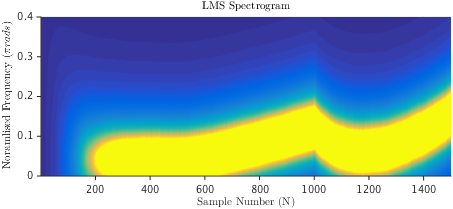
\includegraphics[width=\textwidth]{images/4-2-b-1.png}
		\label{fig:4-2-b-1}
		\caption{Spectrogram of the FM signal, generated using the CLMS algorithm weights}
	\end{subfigure}%
	
	\begin{subfigure}[b]{0.7\textwidth}
		\resizebox{\textwidth}{!}{\input{matlabimages/4-2-b-2.tikz}}
		\label{fig:4-2-b-2}
		\caption{Real and Imaginary parts of the AR(1) weight over time.}
	\end{subfigure}
	\caption{}
	\label{fig:4-2-b}
\end{figure}

Unlike fig~\ref{fig:q4_2_a}, the spectrogram generated here allows us to see into the PSD over time. As such, we can clearly see the a linear PSD, centered around $0.05\pi$ from $N=0:500$. From $N=500:1000$, the PSD linearly increases from $0.05\pi$ to around $0.1\pi$. For the last segment, a parabolic shape is shown. It's interesting to now that between $N=1000:1200$, the CLMS system is converging towards the correct weights, and therefore the parabola is of a strange shape. 

\paragraph{Effect of $\mu$ on the Spectrogram.} As the convergence of the weights, and therefore the estimation of the PSD, is dependant on the learning rate $\mu$, increasing it has the effect of increasing convergence. However, a learning coefficient that is very high will be sensitive to noise - and therefore the resulting PSD will be considerably less smooth.


\begin{figure}[H]
	\centering
	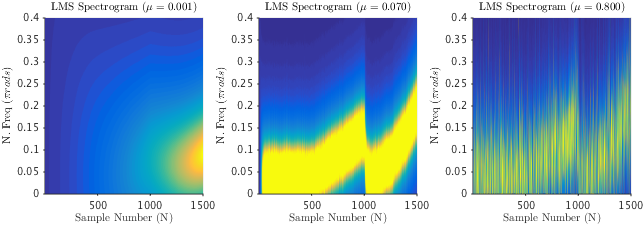
\includegraphics[width=0.7\textwidth]{images/4-2-b-3.png}
	\label{fig:4-2-b-3}
	\caption{Effect of $\mu$ on the LMS Spectrogram}
\end{figure}%


\subsection{A Real Time Spectrum Analyser Using Least Mean Square}

The LMS algorithm can also be used to carry out a real-time spectrum analyser on an input. In every situation used previously, the LMS algorithm find the weights $\textbf{w}(n)$ that can predict the signal $\textbf{y}(n)$ from input $\textbf{x}(n)$. By realising that any signal can be estimated by a linear combinations of $N$ harmonically related sinusoids,

\begin{equation}
\hat{y}(n) = \sum_{k=0}^{N-1}w(k)e^{j2\pi kn/N} \label{eq-4-3-a-yhat}
\end{equation}

one can construct construct a $MA(N)$ algorithm with input 

\begin{equation}
\textbf{x}(n) = \frac{1}{N}\left[1\ \ \ e^{j2\pi n/N}\ \ \ ...\ \ \ e^{j2\pi (N-1)/N}\right]^T
\end{equation}


such that the modified CLMS (DFT-CLMS) algorithm operates on the following principles

\begin{align*}
\hat{y}(n) &= \textbf{w}^H(n)\textbf{x}(n)\\
e(n) &= y(n) - \hat{y}(n) \numberthis \label{eq-4-3-dft-clms}\\
\textbf{w}(n+1) &= \textbf{w}(n) + \mu e^*(n)\textbf{x}(n)
\end{align*}


As the LMS algorithm now searches for weights that will linearly combine harmonic frequecies $\textbf{x}(n)$ to approximate the value of $y(n)$, it should be noted that these weights will approximate the fourier coefficients from the DFT. 

\subsubsection{Least Squares Solution and Comparison to DFT}

To find the optimised weight, $\textbf{w}_0$, that reduces the mean square error $||\textbf{y}-\hat{\textbf{y}}||^2$, set $\Delta_wJ(n)=\textbf{0}$. The result shown in the lecture slides is

\begin{equation}
\textbf{w}_{opt}(n) = arg \min_{w}J(\textbf{w}) = \textbf{R}^{-1}\textbf{p}(n) \label{eq:4-3-a-0}
\end{equation}

where $\textbf{R}$ is the correlation matrix, and $\textbf{p}(n)$ is the cross correlation between $d(n)$ and the input.

In the DFT-LMS algorithm, the input to the algorithm is the matrix $\textbf{F}$.

As such, $\textbf{R}$ and $\textbf{p}$ are defined as 

\begin{align}
\textbf{R} = \textbf{F}^H\textbf{F} \label{eq:4-3-a-1}\\
p = \textbf{F}^H\textbf{y}\label{eq:4-3-a-2}
\end{align}

Substituting \ref{eq:4-3-a-1} and \ref{eq:4-3-a-2} into \ref{eq:4-3-a-0} gives 

\begin{equation}
\textbf{w}_{opt} = \textbf{R}^{-1}\textbf{p} = (\textbf{F}^H\textbf{F})^{-1}\textbf{F}^H\textbf{y}
\end{equation}

\subsubsection{Fourier Transform as a Change of Basis}

When talking about a change of basis, the key concept is changing the axis on which a vector lies. The careful definition of two complimentary dimension spaces and relevant projection matricies is the foundation of basis changing. The previously explored MUSIC algorithm, for instance, was one such change of basis used to distinguish a signal from it's noise. Other examples are Principal Component Analysis (PCA) or Linear Discriminant Analysis (LDA). 

Converting the LMS algorithm to a real-time spectral estimator invokes a different way of thinking about the discrete fourier transform (DFT). By considering a given discrete-time signal of N lengths as a vector in N dimensions (\textit{one dimension for each value of N, i.e. time}), one can define the dimension space of size N $T$. This space is one way of expressing the information held by N-samples by holding one variable for each sample of time.

One can now consider an equally large dimension space, but where each dimension represents a frequency (of size $n/N$, where $n \in [1,N]$). This dimension space can be called $\Omega$, and it holds information on signals by storing the value of each frequency. 

As such, taking the DFT or the IDFT of a signal can be thought of as the conversion between these dimensional subspaces. This process is esentially what is attempted in the DFT-LMS algorithm.

\subsubsection{DFT-CLMS implementation of FM signal}

By using the DFT-CLMS algorithm defined in Equation~\ref{eq-4-3-dft-clms}, the time-frequency plot is created by a heat diagram of the weights $\textbf{w}(n)$.

\begin{figure}[H]
	\centering
	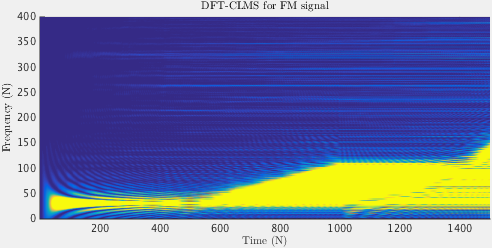
\includegraphics[width=0.7\textwidth]{images/4-3-c.png}
	\caption{Spectrogram of the FM signal calculated with the DFT-CLMS algorithm}
	\label{fig:4-3-c}
\end{figure}%

The spectrum from figure \ref{fig:4-3-c} is only an estimate of the true spectrum of theunderlying signal. Two considerations need to be considered to understand why it is not exact. 

\begin{enumerate}
	\item The DFT-CLMS at steady state only approximates the actual value of $y(n)$ with a linear combination of the harmonically related sinusoidal input $\textbf{x}(n)$. As such, the spectrum in figure \ref{fig:4-3-c} is of the estimated signal $\hat{y}(n)$, defined in equation~\ref{eq-4-3-a-yhat}.
	\item Depending on the value of $\mu$, it should be noted that the values of $w(n)$ do not always approach the exact value of the fourier coefficients. Therefore, the spectrum will not be exact, especially for a rich input signal $y(n)$. From \cite{Widrow1987} the spectrum is at it's most exact when $\mu$ is set to $1$.
\end{enumerate}

\subsubsection{Applying the DFT-CLMS for EEG Data}

The DFT-CLMS algorithm is turned to use on the POz data set used in section 1.4. As figure~\ref{fig:4-3-b-poz} shows, however, the resolution of the algorithm does not allow for identificatio of the SSVP. It is possible, however, to see a sharp line at 50Hz and noise around 7-10Hz, which correspond to the mains line hum and alpha brain waves respectively. 

\begin{figure}[H]
	\centering
	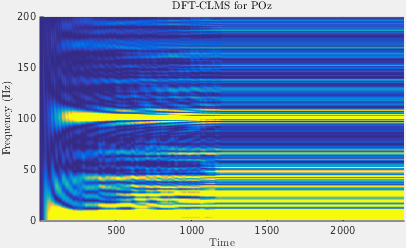
\includegraphics[width=0.7\textwidth]{images/4-3-b-poz.png}
	\label{fig:4-3-b-poz}
	\caption{Spectrogram calculated with the DFT-CLMS algorithm}
\end{figure}%

\paragraph{The limitations of the DFT-CLMS} algorithm are evidences here. As the algorithm converts N-time samples into N-frequency bins, the resolution in the frequency domain is insufficient for this case. A potential work-around is to zero-pad the input, but this adds significant computational load \footnote{This has not been tested by myself, and so cannot be verified}.

\subsubsection{Potential Applications for the DFT-LMS function}

Being able to calculate the DFT on-the-fly is extremely useful in a number of sitations. From the experiments shown here, and those run seperately, the key limitation of the DFT-LMS algorithm is in the resolution of the output. As such, the DFT-LMS can be used in situations where simple spectral comonents need to be tracked (rather than calculated). 

\end{document}